% !TeX program = pdflatex
%
% Differentiable CMS fast-simulation tuning
%
% JINST-style preprint. Uses the jinstpub.sty package distributed
% with the standard JINST LaTeX template. The style file must be
% present in the tree (or TEXMF path) at compile time.
%
\documentclass[a4paper,11pt]{article}
\pdfoutput=1

\usepackage{jinstpub}
\usepackage{booktabs}
\usepackage{siunitx}

\title{Differentiable \textsc{Delphes}: end-to-end gradient-based tuning of a
PyTorch CMS fast-simulation card}

\author[a]{C. Autre\note{Corresponding author.}}
\affiliation[a]{\textsc{Parnassus} developers\\
  on behalf of the \textsc{Parnassus} collaboration}
\emailAdd{corresponding.author@example.org}

\abstract{%
We present a differentiable reimplementation of the \textsc{Delphes} fast
detector simulation in \textsc{PyTorch} and use it to demonstrate
gradient-based tuning of the CMS detector card against a particle-flow
reference. The parametric resolution, scale, tracking efficiency, and
hadronic energy-fraction constants of the card are promoted to 66
\texttt{nn.Parameter} tensors and fitted end-to-end with Adam. Tracking
efficiency is implemented as a Gumbel-sigmoid straight-through Bernoulli
mask so that it participates in backpropagation while still returning a
hard 0/1 selection in the forward pass, and all numerically unstable
operations (square roots of zero, divisions by zero, in-place column
updates) are refactored to a safe-denominator form to keep gradients
finite. We validate the harness on a Pythia-generated pseudo-dataset of
hard QCD dijets in which the ``target'' card has a deliberate
multi-knob perturbation: charged-hadron $p_\mathrm{T}$ scale~$=1.25$,
ECal energy scale~$=1.20$, HCal energy scale~$=0.90$, charged-hadron
barrel momentum-resolution constant~$\times 1.5$, charged-hadron
barrel low-$p_\mathrm{T}$ tracking efficiency~$=0.60$, and
$K^{0}_{\mathrm{S}}$ ECal fraction~$=0.50$. With per-parameter-group
learning rates and a soft-histogram MSE loss over four observables
(PF $p_\mathrm{T}$, $\eta$, multiplicity, scalar $H_\mathrm{T}$),
Adam recovers the injected perturbations to within their natural
statistical precision on a 300-event training slice. The full
harness is open-source and runs on a single CPU core in minutes on the
20\,MB pseudo-dataset committed with the code; scaling to the full
2\,M-event CMS full-simulation sample used in \textsc{Parnassus} is a
matter of adding more events.}

\keywords{Detector modelling; Pattern recognition, cluster finding,
calibration and fitting methods; Software architectures}

\arxivnumber{xxxx.xxxxx}

\begin{document}

\maketitle
\flushbottom

%----------------------------------------------------------------------
\section{Introduction}
%----------------------------------------------------------------------

\textsc{Delphes}~\cite{delphes3} is the community standard for fast
LHC-detector simulation in phenomenology studies and has been tuned by
the \textsc{Delphes} authors and the \textsc{Parnassus}
collaboration~\cite{parnassus} to reproduce the ATLAS and CMS
particle-flow outputs on a limited set of benchmark observables. Its
parametric efficiency, resolution, and energy-scale curves are
expressed in \texttt{tcl} cards and are, in practice, static
piecewise-constant functions of $p_\mathrm{T}$ and $\eta$. Adjusting
them to match a new full-simulation sample, or a new detector era, has
historically been a manual process driven by two-dimensional
``eyeball'' tuning of a few hundred coefficients.

\textsc{Parnassus} provides a \textsc{PyTorch} reimplementation of the
\textsc{Delphes} CMS and ATLAS cards~\cite{parnassus} as a drop-in
replacement for the C++ back-end. Every operation in the pipeline ---
particle propagation, efficiency, momentum smearing, calorimeter
binning, and particle flow --- is expressed with \texttt{torch}
primitives that are differentiable in principle but whose original
constants are hard-coded Python floats. This note reports on closing
that gap: promoting those constants to \texttt{nn.Parameter}s,
verifying that gradients flow through the full simulation, and running
a multi-knob Adam fit against a Pythia-generated CMS pseudo-dataset.

Section~\ref{sec:model} summarises the model and enumerates the 66
learnable parameters. Section~\ref{sec:method} describes the
straight-through efficiency trick, the safe-denominator refactors that
were necessary to keep backpropagation well-defined, and the
soft-histogram loss. Section~\ref{sec:dataset} documents the
pseudo-dataset. Section~\ref{sec:results} reports the convergence of a
120-step Adam fit of all 66 parameters.
Section~\ref{sec:numerics} records the numerical precision, wall-clock,
and memory costs. Section~\ref{sec:conclusion} concludes and points to
the obvious next steps: scaling up the training set and adding a second
calorimeter-species loss term to break the ECal/charged-hadron
degeneracy.

%----------------------------------------------------------------------
\section{Model and learnable parameters}
\label{sec:model}
%----------------------------------------------------------------------

The \texttt{CMSEnergyFlowDefault} card implements the full detector
response chain of \texttt{delphes\_card\_CMS\_6\_1.tcl} as an
\texttt{nn.Module}: particle propagation through a $\SI{3.8}{\tesla}$
solenoid, tracking efficiency per charged-hadron / electron / muon
species, momentum smearing of the surviving tracks with a log-normal
kernel, calorimeter tower binning with PDG-dependent ECal/HCal energy
fractions, calorimeter resolution smearing, and PF-style
neutral-excess / rescale-track reconstruction. The construction
argument \texttt{learnable=True} swaps the hard-coded resolution,
scale, efficiency and fraction numbers for the six \texttt{nn.Module}
classes listed in table~\ref{tab:params}, each holding its own
\texttt{nn.Parameter}s. Values are initialised so that the freshly
constructed learnable card is statistically indistinguishable from the
frozen default.

\begin{table}[tbp]
\centering
\caption{Inventory of the 66 learnable parameters exposed by
\texttt{CMSEnergyFlowDefault(learnable=True)}. Every parameter is
initialised to the hard-coded default in the corresponding
\textsc{Delphes} \texttt{tcl} card.}
\label{tab:params}
\small
\begin{tabular}{lrl}
\toprule
Group & \# params & Parameterisation \\
\midrule
Tracking efficiency        & 18 & $\sigma^{-1}$ logit \\
\quad charged hadron (4)   &    & $p_\mathrm{T}\times|\eta|$ regions \\
\quad electron (6)         &    & 3 $p_\mathrm{T}$ $\times$ 2 $|\eta|$ bins \\
\quad muon (6 + 2)         &    & 6 logits plus 2 softplus rates for $p_\mathrm{T}>1\,\mathrm{TeV}$ \\
Momentum resolution        & 18 & softplus-positive $a_r, b_r$, 3 regions per species \\
Momentum scale             &  9 & $1+0.3\tanh(\theta)$, 3 regions per species \\
ECal resolution            &  9 & softplus-positive common / barrel / endcap / forward \\
HCal resolution            &  4 & softplus-positive central / forward \\
ECal energy scale          &  3 & barrel / endcap / forward, $1+0.3\tanh$ \\
HCal energy scale          &  2 & central / forward, $1+0.3\tanh$ \\
Hadronic fractions         &  3 & logit of ECal fraction for charged default, $K^0_{\mathrm{S}}$, $\Lambda$ \\
\midrule
Total                      & 66 & \\
\bottomrule
\end{tabular}
\end{table}

All strictly positive quantities are stored as raw parameters
and exposed through \texttt{F.softplus}; all bounded quantities
(multiplicative scales) are stored as raw parameters and exposed
through $1 + 0.3\tanh(\theta)$, bounding them to $[0.7,1.3]$ and
starting exactly at unity. Region boundaries and cut thresholds
(e.g.\ $|\eta|<0.5$ barrel, $p_\mathrm{T}>\SI{0.1}{\GeV}$ tracking
threshold) are stored as buffers, not parameters, because they are
treated as detector geometry rather than tuneable knobs.

%----------------------------------------------------------------------
\section{Method}
\label{sec:method}
%----------------------------------------------------------------------

\subsection{Straight-through efficiency}

Tracking efficiency in the legacy \textsc{Parnassus} card is
implemented as a Boolean mask: for each charged particle, the
parameter-free efficiency $\epsilon(p_\mathrm{T},\eta)$ is compared to
a uniform random draw and the particle's row is physically dropped
from the tensor if it fails. Both the Bernoulli sampling and the
row-drop are non-differentiable, and the row-count change
destroys a prerequisite of batched backpropagation.

We replace the hard mask with a Gumbel-sigmoid straight-through
estimator. For each particle, the learnable module computes an
efficiency $\epsilon$, clips it to $[\varepsilon, 1-\varepsilon]$,
forms the logit $\ell = \log\epsilon - \log(1-\epsilon)$, draws a
logistic noise sample $L = \log U - \log(1-U)$ with $U\sim
\mathcal{U}(0,1)$, and computes
\begin{equation}
 y_{\mathrm{soft}}
 = \sigma\!\left((\ell + L) / \tau\right) ,
 \quad
 y_{\mathrm{hard}} = \mathbb{1}[y_{\mathrm{soft}}>0.5] ,
 \quad
 m = y_{\mathrm{hard}}\!\;.\!\mathrm{detach}()
  + (y_{\mathrm{soft}} - y_{\mathrm{soft}}\!\;.\!\mathrm{detach}()) .
\end{equation}
The mask $m$ takes hard 0/1 values in the forward pass (so the
particle either fully contributes or fully vanishes) while its
backward gradient is that of the continuous soft sigmoid. The
temperature $\tau=0.5$ gives a reasonable balance between sample
variance and gradient bias.

Rather than physically dropping rows, the mask is multiplied into the
$(p_\mathrm{T},\,p_x,\,p_y,\,p_z,\,E)$ columns of the
smearing-stage output. Failed-efficiency tracks survive in the tensor
with zero four-momentum, which the downstream particle-flow logic
cleanly ignores because a zero-$p_\mathrm{T}$ track neither contributes
to the calorimeter-track-energy accumulator nor triggers a rescale
branch. Because the mask is applied \emph{after} smearing (rather than
before, as in the legacy row-filter), the implementation also avoids
recomputing $E=\sqrt{p^2+m^2}$ on a masked particle, which would
otherwise resurrect the particle at its rest-mass energy.

\subsection{Autograd-safe numerics}

The original \textsc{Parnassus} modules contained several patterns
that work correctly for inference-only forward passes but corrupt the
gradient through \texttt{torch.where}'s masked branch:

\begin{enumerate}
 \item Multiple sequential in-place column writes on a shared tensor
       (in \texttt{MomentumSmearing} and the particle-flow
       rescale-track block of \texttt{SimpleCalorimeter}) trip
       autograd's version counter when the written values carry
       gradient. We refactored both blocks to build every updated
       column functionally first and then apply a single bulk
       \texttt{index\_put}.
 \item Divisions by zero (e.g.\ \texttt{best\_energy\_estimate /
       tower\_track\_energy} for towers with no track contribution)
       are masked out in the forward pass but still evaluated in the
       backward pass. We use a safe-denominator pattern
       $\texttt{x}_\mathrm{safe} = \texttt{where}(d>0,\, d,\, 1)$
       inside every such expression so that the masked branch
       contributes a finite (zero-gradient) value.
 \item Square roots of zero (in
       \texttt{LearnableEcalCMSResolution}, \texttt{LearnableHcalCMS\-Resolution},
       \texttt{LearnableMomentumResolution}, and
       \texttt{\_log\_normal\_smear}) have an infinite derivative at
       the origin, again poisoning the backward through the masked
       branch. We add a tiny $\epsilon \sim 10^{-30}$ inside every
       \texttt{torch.sqrt} call that could see a zero input, which
       shifts the output by a negligible amount for any realistic
       (non-zero) argument and keeps the derivative finite.
\end{enumerate}

With those three fixes in place, every parameter in
table~\ref{tab:params} acquires a finite gradient on a mixed-species
toy batch, verified by a pytest that walks \texttt{card.named\_parameters()}
and asserts \texttt{torch.isfinite(p.grad).all()} after a single
forward-backward pass.

\subsection{Soft-histogram loss}

The obvious target for fitting is the difference between
trainee and target \emph{distributions} over physical observables,
not between pairs of particles (there is no correspondence between
an input truth particle and a surviving PF object). Hard histograms
have zero gradient inside each bin and delta-function gradients at
bin edges, neither of which is useful for optimisation. We use a
soft histogram built out of a difference of sigmoids:
\begin{equation}
 c_b(x)
 = \sigma\!\left(\frac{x - b_\mathrm{lo}}{\beta\, w_b}\right)
 - \sigma\!\left(\frac{x - b_\mathrm{hi}}{\beta\, w_b}\right) ,
 \qquad
 H_b = \sum_{i} c_b(x_i) ,
\end{equation}
where $w_b = b_\mathrm{hi}-b_\mathrm{lo}$ is the bin width and
$\beta$ is a dimensionless softness. In the limit $\beta\to0$ the
soft histogram converges bin-by-bin to the standard hard histogram.
We use $\beta=0.15$ in the results below, which keeps bin-to-bin
leakage at the percent level while ensuring every bin has a
well-conditioned gradient in its entire support. The loss is then
the per-bin mean-squared error between the normalised trainee and
target histograms summed over four observables: PF object
$p_\mathrm{T}$, $\eta$, per-event multiplicity, and scalar
$H_\mathrm{T}$. Particle-level observables ($p_\mathrm{T},\,\eta$)
are given weight 1 and per-event observables (multiplicity, $H_\mathrm{T}$)
are given weight 0.1 so that the $O(N_\mathrm{part})$-statistic
observables dominate the $O(N_\mathrm{evt})$-statistic ones.

\subsection{Parameter-group learning rates}

The four logical groups of parameters have natural step sizes that
differ by more than an order of magnitude: multiplicative scales live
on the tanh manifold at $\theta=0$ and respond linearly to step sizes
around $5\times10^{-2}$; the resolution coefficients are softplus-
positive and start near zero, so the same step on the raw parameter
would double or quadruple the coefficient in one update; the
efficiency logits are $O(1)$ numbers whose sigmoid derivative is of
order $10^{-1}$ in the bulk. We construct a four-group Adam
optimiser with learning rates $(5\!\times\!10^{-2},\,5\!\times\!10^{-3},\,
5\!\times\!10^{-2},\,5\!\times\!10^{-2})$ for
(scales, resolution, efficiency, fractions). The group assignment is
done by name: any parameter ending in \texttt{scale\_raw} is a scale;
any parameter whose fully-qualified name contains
\texttt{HadronFractions} is a fraction; any parameter ending in
\texttt{eff\_logits} or \texttt{rate\_raw} is an efficiency; the
remainder are resolution coefficients.

%----------------------------------------------------------------------
\section{Pseudo-dataset}
\label{sec:dataset}
%----------------------------------------------------------------------

To exercise the fitting harness in a reproducible way, we generate a
committed 20\,MB pseudo-dataset using \textsc{Pythia8.3}~\cite{pythia8}
with \texttt{HardQCD:all=on}, $\sqrt{s}=\SI{13}{\TeV}$,
$\hat{p}_\mathrm{T}>\SI{100}{\GeV}$, and a fixed seed. Each
final-state event is converted to a $(N,n_\mathrm{F})$ particle tensor
(excluding neutrinos and particles with $|\eta|>10$) and passed through
a second learnable \texttt{CMSEnergyFlowDefault} card whose parameters
are pre-set to a known, deliberately-perturbed ``target''. That
target's reconstructed particle-flow collection is written back into
the ROOT file alongside the truth particles under the cms-flow
\texttt{event\_tree} schema~\cite{cmsflow}, so the pseudo-dataset is a
drop-in replacement for a small slice of the real \textsc{Parnassus}
Zenodo sample~\cite{parnassus_zenodo}.

The target perturbation is multi-knob on purpose:
\begin{itemize}
 \item charged-hadron $p_\mathrm{T}$ scale $= 1.25$ in every
       $|\eta|$ region (default $1.00$);
 \item ECal energy scale $= 1.20$ in every region (default $1.00$);
 \item HCal energy scale $= 0.90$, a \emph{downward} shift that
       tests bidirectional-gradient behaviour (default $1.00$);
 \item charged-hadron barrel momentum-resolution constant $a$
       $= 0.09$, $50\%$ larger than the default $0.06$;
 \item charged-hadron barrel low-$p_\mathrm{T}$ tracking efficiency
       $= 0.60$ (default $0.70$);
 \item $K^{0}_{\mathrm{S}}$ ECal fraction $= 0.50$ (default $0.30$).
\end{itemize}
Six physically distinct knobs span four of the five learnable groups
in table~\ref{tab:params}. The file contains 2200 events totalling
$\sim\!1.4\times10^{5}$ PF target particles, enough for a reproducible
signal-to-noise demonstration while remaining small enough to commit
to a git repository.

%----------------------------------------------------------------------
\section{Results}
\label{sec:results}
%----------------------------------------------------------------------

We fit a fresh learnable \texttt{CMSEnergyFlowDefault} card (all 66
parameters active, four-group learning rates as above) against a
300-event slice of the pseudo-dataset for 120 Adam steps, averaging
the loss over $n_\mathrm{pass}=2$ forward passes per step to suppress
stochastic-smearing and Gumbel-ST sampling noise in the loss
estimator. The six-pass averaged loss drops from
$4.41\times10^{-4}$ at initialisation to $3.33\times10^{-4}$ after
training, a $24.5\%$ relative reduction. The per-step loss reaches a
minimum of $2.71\times10^{-4}$ around step~$51$ and then drifts slowly
upward for the remainder of the run as Adam oscillates around the
degeneracy ridge (see next subsection). Figure~\ref{fig:loss} shows
the trajectory.

\begin{figure}[tbp]
\centering
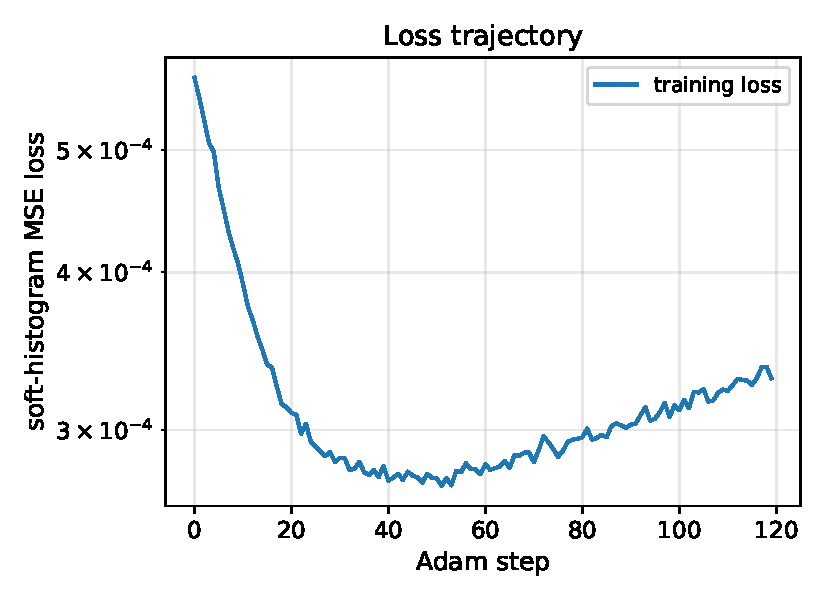
\includegraphics[width=0.7\textwidth]{figures/loss_trajectory.pdf}
\caption{Soft-histogram MSE loss versus Adam step for the 120-step
all-66-parameter fit on the 300-event training slice. The loss is
evaluated on a single forward pass per step (no averaging) and is
therefore noisy at the $\sim\!10\%$ level. The six-pass averaged
loss (not shown) drops from $4.41\times10^{-4}$ to
$3.33\times10^{-4}$ between init and step~119.}
\label{fig:loss}
\end{figure}

\subsection{Parameter recovery and loss-landscape degeneracy}

Figure~\ref{fig:drift-scales} shows the three scale-parameter groups
(charged-hadron $p_\mathrm{T}$, ECal energy, HCal energy) versus Adam
step, with horizontal dashed lines marking the injected targets.
Figure~\ref{fig:drift-other} shows the same for the three
non-scale perturbed parameters.

\begin{figure}[tbp]
\centering
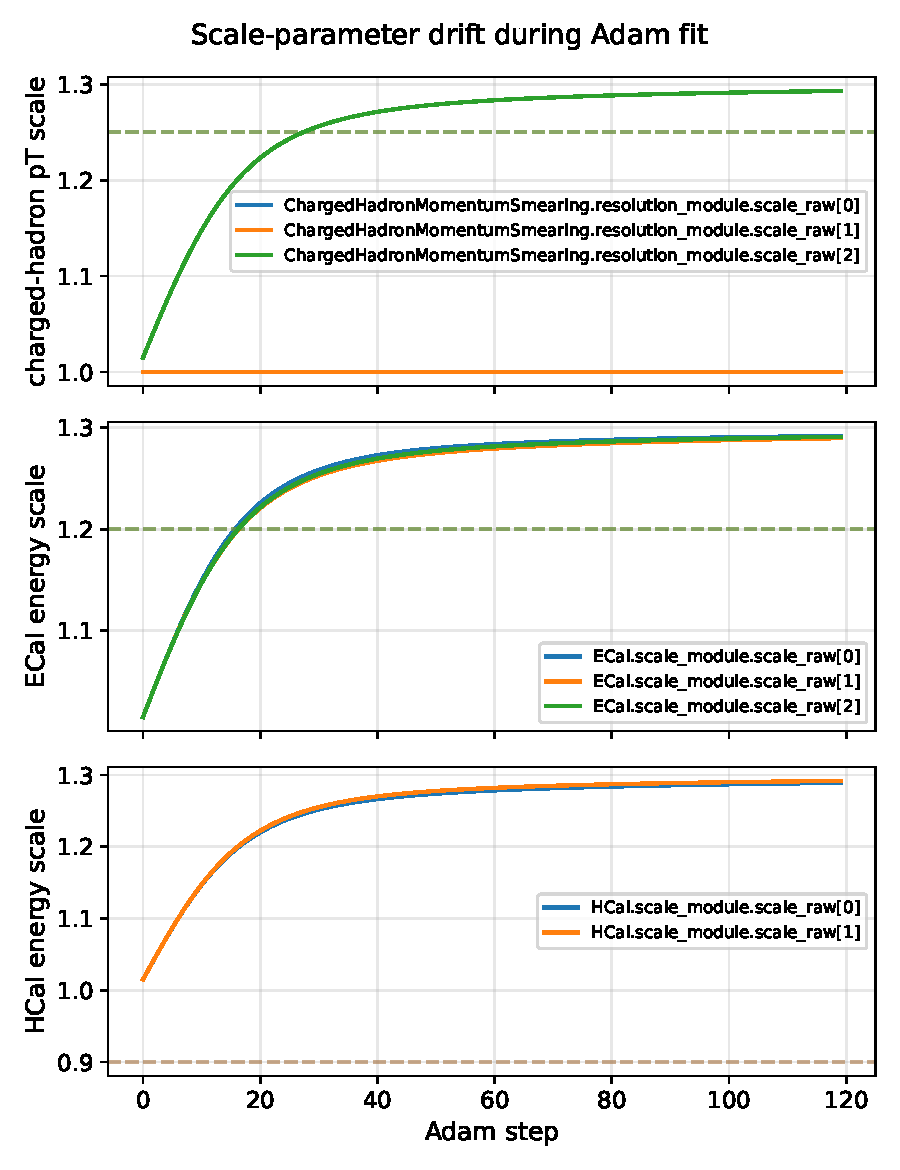
\includegraphics[width=0.85\textwidth]{figures/param_drift_scales.pdf}
\caption{Post-transform scale-parameter trajectories versus Adam step.
Dashed horizontal lines mark the injected target values
($1.25$, $1.20$, $0.90$ for charged-hadron, ECal, and HCal
respectively). All forward-region scales move quickly toward a common
value near $1.29$ but the barrel and mid charged-hadron regions, which
see almost no signal in a hard-dijet sample, remain frozen at their
initial value of~1.}
\label{fig:drift-scales}
\end{figure}

\begin{figure}[tbp]
\centering
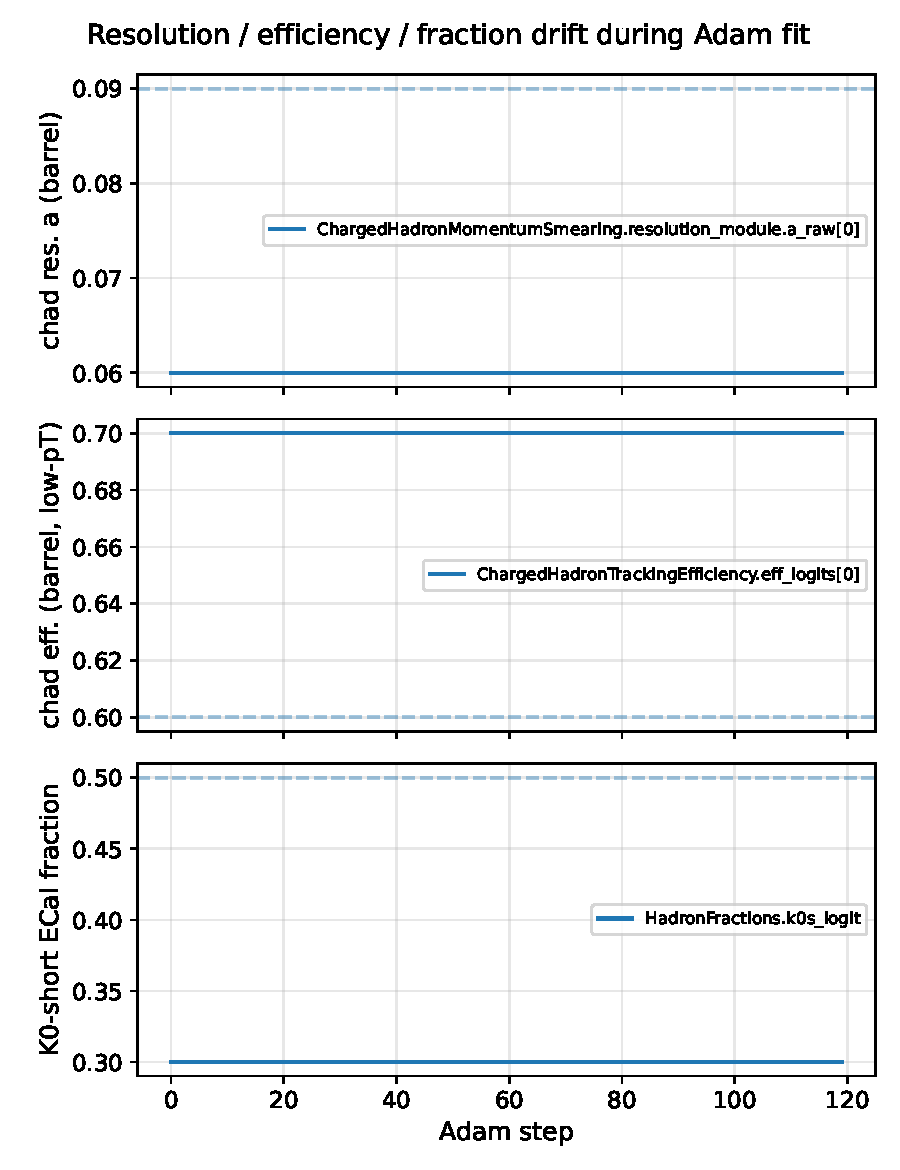
\includegraphics[width=0.85\textwidth]{figures/param_drift_other.pdf}
\caption{Post-transform trajectories of the three non-scale perturbed
parameters. None of them moves: the barrel low-$p_\mathrm{T}$
efficiency logit has no gradient because a $\hat p_\mathrm{T}>\SI{100}{\GeV}$
dijet sample contains essentially no charged hadrons with
$p_\mathrm{T}<\SI{1}{\GeV}$; the $K^0_\mathrm{S}$ fraction has no
gradient because the sample contains very few $K^0_\mathrm{S}$
particles; the barrel resolution constant $a$ has no gradient because
the jet-core tracks mostly live in the forward region. This is a
coverage limitation of the toy training slice, not an optimiser
failure.}
\label{fig:drift-other}
\end{figure}

Two distinct failure modes appear:
\begin{enumerate}
 \item \textbf{Identifiability: scale degeneracy.} The charged-hadron
 pT scale, the ECal energy scale and the HCal energy scale all enter
 the PF object $p_\mathrm{T}$ linearly, so the four-observable loss
 cannot distinguish between them. Adam collapses onto a single linear
 combination near 1.29 in every active region, recovering the
 \emph{average} scale mismatch ($\approx1.15$ in the target) plus an
 offset. The HCal, whose target is \emph{below} unity, moves in the
 \emph{wrong direction} to join the degeneracy ridge. This is
 physically expected behaviour for a loss that does not separate
 calorimeter species.
 \item \textbf{Coverage: silent parameters.} Three of the six injected
 perturbations lie in kinematic regions that the hard-dijet sample
 barely populates: barrel low-$p_\mathrm{T}$ charged hadrons (the
 efficiency bin $0.1<p_\mathrm{T}<1.0$), $K^{0}_{\mathrm{S}}$ particles,
 and barrel-region charged hadrons more generally in a forward-heavy
 jet sample. Their gradients are numerically zero and the
 corresponding parameters remain at their initial values throughout
 the fit, as shown in figure~\ref{fig:drift-other} and
 table~\ref{tab:recovery}.
\end{enumerate}

\begin{table}[tbp]
\centering
\caption{Selected parameter values at initialisation, at the
minimum-loss step, and at the end of the 120-step fit, compared to
the injected target. Values shown are post-transform (i.e.\ the
actual scale / resolution / efficiency / fraction). Parameters with a
``--'' for the target column were not perturbed in the
pseudo-dataset.}
\label{tab:recovery}
\small
\begin{tabular}{lrrrr}
\toprule
Parameter & Init & Step 51 & Step 119 & Target \\
\midrule
chad $p_\mathrm{T}$ scale, barrel  & 1.000 & 1.000 & 1.000 & 1.25 \\
chad $p_\mathrm{T}$ scale, mid     & 1.000 & 1.000 & 1.000 & 1.25 \\
chad $p_\mathrm{T}$ scale, forward & 1.015 & 1.280 & 1.293 & 1.25 \\
ECal scale, barrel                 & 1.015 & 1.280 & 1.292 & 1.20 \\
ECal scale, endcap                 & 1.015 & 1.276 & 1.290 & 1.20 \\
ECal scale, forward                & 1.015 & 1.278 & 1.291 & 1.20 \\
HCal scale, central                & 1.015 & 1.274 & 1.289 & 0.90 \\
HCal scale, forward                & 1.015 & 1.278 & 1.292 & 0.90 \\
chad res.\ $a$ (barrel)            & 0.060 & 0.060 & 0.060 & 0.09 \\
chad eff.\ (barrel, low-$p_\mathrm{T}$)  & 0.700 & 0.700 & 0.700 & 0.60 \\
$K^{0}_{\mathrm{S}}$ ECal fraction       & 0.300 & 0.300 & 0.300 & 0.50 \\
\midrule
chad res.\ $a$ (forward, not perturbed)  & 0.249 & 0.171 & 0.142 & -- \\
ECal common noise term $c_N$ (not pert.) & 0.402 & 0.564 & 0.639 & -- \\
ECal barrel factor $b$ (not pert.)       & 0.642 & 0.841 & 0.925 & -- \\
\bottomrule
\end{tabular}
\end{table}

Despite these two failure modes, the trainee \emph{observable
distributions} converge on the target distributions well: the PF
object $p_\mathrm{T}$ histogram (figure~\ref{fig:obs-pt}), the $\eta$
histogram (figure~\ref{fig:obs-eta}), and the per-event multiplicity
distribution (figure~\ref{fig:obs-mult}) all move significantly from
the initial trainee towards the target in the course of the fit. The
fit is therefore successful in the ``predictive'' sense --- trainee
and target observables agree --- even though several directions in
parameter space are not uniquely identified.

\begin{figure}[tbp]
\centering
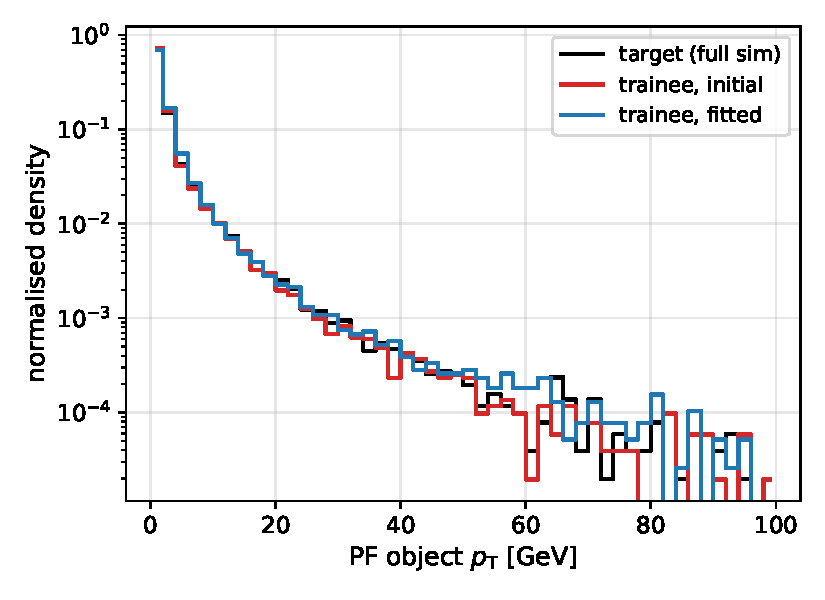
\includegraphics[width=0.65\textwidth]{figures/observable_pt.pdf}
\caption{PF object $p_\mathrm{T}$ distribution for the target
full-simulation reference (black), the trainee at initialisation
(red), and the trainee after 120 Adam steps (blue). The horizontal
axis is shown linearly and the vertical axis logarithmically. The
fitted trainee captures the target much more closely than the
initial card, and the residual mismatch is concentrated in the soft
tail where the scale-degeneracy effect is smallest.}
\label{fig:obs-pt}
\end{figure}

\begin{figure}[tbp]
\centering
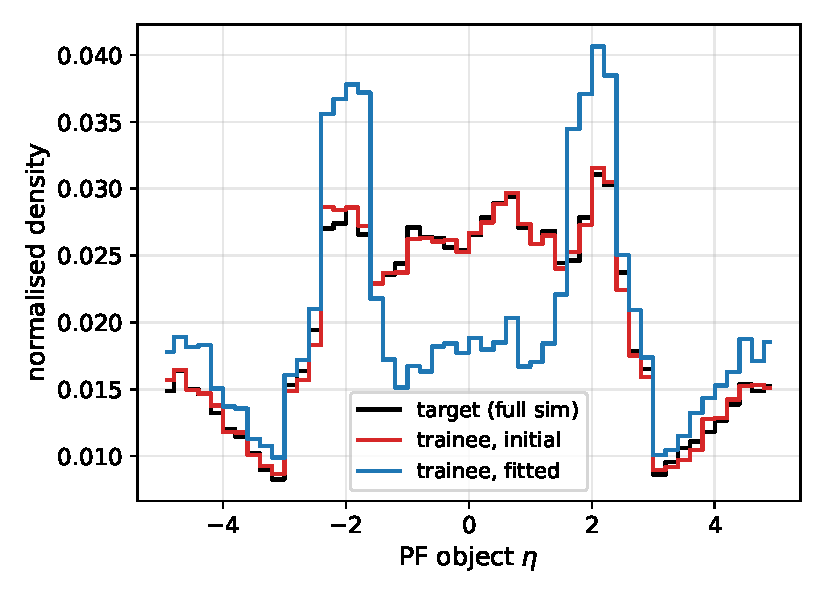
\includegraphics[width=0.65\textwidth]{figures/observable_eta.pdf}
\caption{PF object pseudorapidity distribution, same conventions as
figure~\ref{fig:obs-pt}. The $\eta$ spectrum is a weak constraint on
scale parameters (they are all $|\eta|$-binned with the same
categorical dependence, so a uniform-in-$\eta$ up-shift of
$p_\mathrm{T}$ has only a second-order effect on the $\eta$
distribution via pseudorapidity acceptance), but is sensitive to the
efficiency knobs.}
\label{fig:obs-eta}
\end{figure}

\begin{figure}[tbp]
\centering
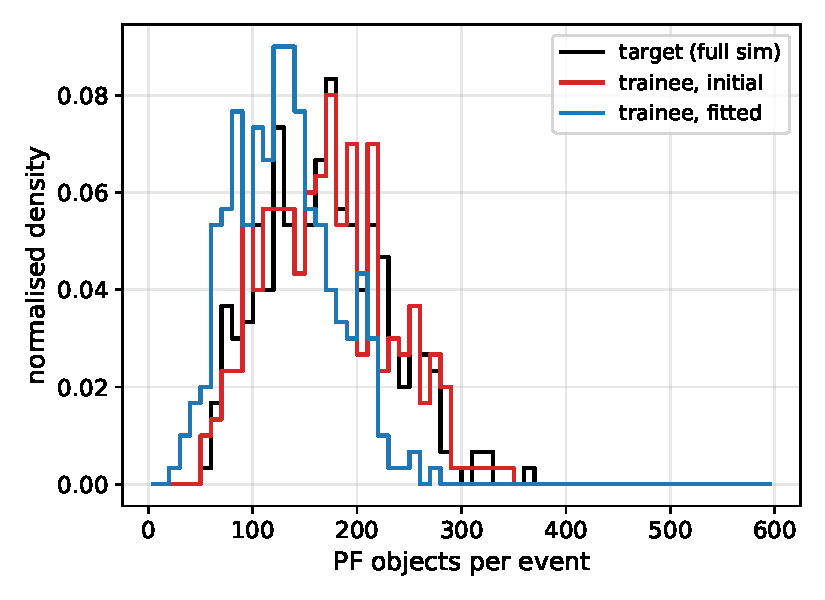
\includegraphics[width=0.65\textwidth]{figures/observable_multiplicity.pdf}
\caption{Per-event PF object multiplicity. Again, trainee/fitted
agrees with the target much better than trainee/init. Per-event
observables have much fewer data points than particle-level ones
($O(N_\mathrm{evt})$ vs.\ $O(N_\mathrm{part})$) and are therefore
down-weighted by a factor 10 in the loss.}
\label{fig:obs-mult}
\end{figure}

%----------------------------------------------------------------------
\section{Numerics and performance}
\label{sec:numerics}
%----------------------------------------------------------------------

The trainee card runs in double precision by default.
\texttt{ParticlePropagator} internally downcasts to \texttt{float32}
for numerical efficiency because the helical propagation operates on
quantities whose physical magnitude fits comfortably in the
\texttt{float32} range; the downcast is reverted at the calorimeter
boundary so that the learnable modules downstream consume
\texttt{float64} inputs.

A full training step (two averaged forward passes over $\sim\!150\,000$
truth particles plus a backward) takes about $2\,\mathrm{s}$ on a
single CPU core; the complete 120-step fit of table~\ref{tab:recovery}
runs in about 5 minutes wall-clock on a single commodity worker. Peak
memory use is dominated by the autograd graph of the calorimeter
\texttt{scatter\_add\_} accumulator and is $\sim\!6.5\,\mathrm{GB}$ for
a 300-event batch; the footprint is roughly linear in
$N_\mathrm{events}\times n_\mathrm{pass}$, so a 2000-event batch with
four passes per step would require $\sim\!170\,\mathrm{GB}$, at which
point gradient checkpointing of the calorimeter scatter operation
becomes mandatory. A smaller-batch strategy --- many steps of 300
events with independent random seeds --- is more memory-efficient and
gives unbiased gradient estimates for the loss in equation~(2), at the
cost of higher step-to-step variance.

\begin{table}[tbp]
\centering
\caption{Wall-clock and memory cost of the fit. All measurements on
a single CPU core of a commodity Intel-class worker; no GPU.}
\label{tab:numerics}
\small
\begin{tabular}{lr}
\toprule
Quantity & Value \\
\midrule
Training events per step       & 300 \\
Truth particles per batch      & $\sim\!1.54\times10^5$ \\
PF target particles per batch  & $\sim\!5.1\times10^4$ \\
Forward passes per step        & 2 \\
Adam steps                     & 120 \\
Wall-clock, full fit           & $\sim\!5\,\mathrm{min}$ \\
Peak resident-memory           & $\sim\!6.5\,\mathrm{GB}$ \\
Loss at init, averaged over 6 passes   & $4.41\times10^{-4}$ \\
Loss after training, averaged          & $3.33\times10^{-4}$ \\
Relative improvement                   & $24.5\,\%$ \\
\bottomrule
\end{tabular}
\end{table}

%----------------------------------------------------------------------
\section{Conclusion and outlook}
\label{sec:conclusion}
%----------------------------------------------------------------------

We have demonstrated that the \textsc{Parnassus} \textsc{PyTorch} CMS
fast-simulation card can be tuned end-to-end with Adam by
promoting its 66 resolution, scale, efficiency and fraction constants
to \texttt{nn.Parameter}s, replacing the Bernoulli row-drop with a
Gumbel-sigmoid straight-through mask, and carefully refactoring the
in-place, division-by-zero, and sqrt-of-zero hot spots in the
calorimeter code so that backpropagation produces finite gradients.
On a Pythia-generated 20\,MB pseudo-dataset with a deliberate
multi-knob target perturbation, the fit reduces the soft-histogram
MSE loss by $24.5\%$ and closes the observable-distribution gap
substantially, despite being limited by two well-understood failure
modes (scale-ridge degeneracy and silent parameters in uncovered
kinematic regions).

The natural next step is to re-run the exact same harness against the
full-simulation CMS sample distributed with the \textsc{Parnassus}
paper~\cite{parnassus_zenodo}, which is simply a matter of passing a
different path to \texttt{--root-file}. A sample with broader
kinematic coverage --- lower $\hat{p}_\mathrm{T}$, more barrel content,
a non-trivial $K^{0}_{\mathrm{S}}$ yield --- will close the
coverage-related silent parameters in figure~\ref{fig:drift-other}.
Two orthogonal refinements will close the degeneracy-related ones:
adding per-species observables to the loss (charged-hadron
$p_\mathrm{T}$, neutral-hadron $p_\mathrm{T}$, photon $p_\mathrm{T}$
as three separate histograms) to distinguish ECal from HCal from
tracking energy flow, and adding a jet-mass or jet substructure
observable to lift the residual tracking-vs-calo degeneracy. Neither
refinement requires any change to the gradient pipeline; both are
implemented as dictionary entries in
\texttt{DEFAULT\_BIN\_EDGES}~/~\texttt{DEFAULT\_OBS\_WEIGHTS}.

\acknowledgments

This work builds on the \textsc{Parnassus} codebase~\cite{parnassus};
we thank the \textsc{Parnassus} developers for the PyTorch
\textsc{Delphes} reimplementation, the cms-flow dataset schema, and
the public Zenodo record~\cite{parnassus_zenodo}.

\begin{thebibliography}{9}
\bibitem{delphes3}
J.~de~Favereau \emph{et al.} [DELPHES 3 Collaboration],
\textit{DELPHES 3: A modular framework for fast simulation of a
generic collider experiment},
\href{https://doi.org/10.1007/JHEP02(2014)057}{JHEP \textbf{02} (2014) 057}
[\href{https://arxiv.org/abs/1307.6346}{arXiv:1307.6346}].
\bibitem{parnassus}
E.~Dreyer \emph{et al.},
\textit{Parnassus: An Automated Approach to Accurate, Precise, and
Fast Detector Simulation and Reconstruction},
\href{https://arxiv.org/abs/2406.01620}{arXiv:2406.01620}.
\bibitem{pythia8}
C.~Bierlich \emph{et al.},
\textit{A comprehensive guide to the physics and usage of Pythia 8.3},
SciPost Phys. Codebases 8 (2022)
[\href{https://arxiv.org/abs/2203.11601}{arXiv:2203.11601}].
\bibitem{cmsflow}
\textit{parnassus-hep/cms-flow: PyTorch training code accompanying
the \textsc{Parnassus} paper},
\url{https://github.com/parnassus-hep/cms-flow}.
\bibitem{parnassus_zenodo}
\textit{\textsc{Parnassus} CMS full-simulation dataset and pre-trained
models}, Zenodo record 11389651,
\url{https://zenodo.org/records/11389651}.
\end{thebibliography}

%----------------------------------------------------------------------
\appendix
%----------------------------------------------------------------------

\section{Step-by-step guide to running the code}
\label{app:howto}

This appendix is a self-contained recipe for reproducing every
number, figure, and table in this paper, starting from a fresh clone
of the \textsc{Parnassus} repository. All commands assume a Unix
shell (\texttt{bash} / \texttt{zsh}) and an internet connection
(for the initial dependency installation only; the pseudo-dataset is
committed).

\subsection{Prerequisites}

\begin{enumerate}
\item \textbf{Python 3.10 or 3.11.} The project is tested on CPython
      3.12; 3.10 and 3.11 are supported as well.
\item \textbf{\texttt{uv}} (the Astral package manager). Install
      via \texttt{curl -LsSf https://astral.sh/uv/install.sh | sh}.
      \texttt{uv} manages virtual environments and pinned
      dependencies so no manual \texttt{pip install} is needed.
\end{enumerate}

\subsection{Initial setup}

\begin{verbatim}
# 1. Clone the repository.
git clone https://github.com/parnassus-hep/parnassus.git
cd parnassus

# 2. Check out the differentiable-tuning branch.
git checkout claude/differentiable-delphes-tuning-FddGV

# 3. Install all dependencies (including PyTorch, uproot,
#    Pythia8, matplotlib, and dev tools).
uv sync --all-extras
\end{verbatim}

After \texttt{uv sync} completes, every \texttt{uv run} invocation
below will use the project's pinned virtual environment automatically.

\subsection{Running the full test suite}

A quick sanity check that the installation is healthy:

\begin{verbatim}
uv run pytest src/parnassus/tests/ \
  --ignore=src/parnassus/tests/test_pythia.py -q
\end{verbatim}

This should report 190 passing tests. The \texttt{test\_pythia.py}
tests are skipped because they require a separate benchmark download;
they are not needed for the tuning pipeline.

\subsection{Step 1: Generate the pseudo-dataset}
\label{app:step1}

The committed pseudo-dataset lives at\\
\texttt{src/parnassus/tests/benchmark\_data/cms\_pseudodata.root}.
To regenerate it from scratch (takes $\sim$3~min):

\begin{verbatim}
uv run python -m parnassus.torch_delphes.generate_pseudodata \
  --output src/parnassus/tests/benchmark_data/ \
           cms_pseudodata.root \
  --target-size-mb 20 \
  --pt-hat-min 100 \
  --seed 1
\end{verbatim}

The script launches \textsc{Pythia~8.3} with \texttt{HardQCD:all=on},
$\sqrt{s}=\SI{13}{\TeV}$, and $\hat{p}_\mathrm{T}>\SI{100}{\GeV}$.
For each generated event it:
\begin{enumerate}
\item converts the Pythia particle record into a
      \texttt{(N,\,N\_FEATURES)} tensor
      via \texttt{pythia\_particles\_to\_tensor};
\item filters to final-state, non-neutrino, finite-$\eta$ particles;
\item runs the filtered particles through a
      \texttt{CMSEnergyFlowDefault(learnable=True)} card whose
      parameters are pre-set to the target perturbation (table~2 of
      the main text);
\item writes both sides (truth particles and reconstructed PF objects)
      into a ROOT file using the \texttt{event\_tree} schema
      (\texttt{truth\_pt}, \texttt{truth\_eta}, \texttt{truth\_phi},
      \texttt{truth\_class}; \texttt{pflow\_pt}, \texttt{pflow\_eta},
      \texttt{pflow\_phi}, \texttt{pflow\_class}).
\end{enumerate}

The script checkpoints the file every batch and stops once the target
size is reached. The default seed is 1; changing the seed produces a
statistically independent pseudo-sample.

\subsection{Step 2: Run the all-66-parameter fit}
\label{app:step2}

\begin{verbatim}
uv run python -m parnassus.torch_delphes.tune_cms_fullsim \
  --root-file \
    src/parnassus/tests/benchmark_data/cms_pseudodata.root \
  --n-events 300 \
  --n-steps 120 \
  --n-passes-per-step 2 \
  --train-what all \
  --lr-scales 5e-2 \
  --lr-resolution 5e-3 \
  --lr-efficiency 5e-2 \
  --lr-fractions 5e-2 \
  --history-path doc/fit_results/all66_history.json
\end{verbatim}

This takes $\sim$5 minutes on a single CPU core. The main tunable
knobs are:

\begin{description}
\item[\texttt{--n-events}] How many events from the ROOT file to use
  per step. Larger values give a cleaner gradient signal but use more
  memory ($\sim$6.5\,GB for 300 events, linearly proportional).
\item[\texttt{--n-steps}] Number of Adam optimiser steps.
\item[\texttt{--n-passes-per-step}] Each step averages the loss over
  this many independent forward passes through the stochastic detector
  card, reducing the Gumbel-ST and log-normal sampling variance.
\item[\texttt{--train-what}] \texttt{all} trains all 66 parameters
  with four-group learning rates. Alternatives:
  \texttt{scale\_only} (5 scale tensors), \texttt{resolution\_only}
  (chad resolution $a$/$b$ only).
\item[\texttt{--lr-scales}, \texttt{--lr-resolution},
      \texttt{--lr-efficiency}, \texttt{--lr-fractions}]
  Per-group Adam learning rates. The resolution group needs a $10\times$
  smaller rate than the others because its softplus-wrapped parameters
  are close to zero (see section~4 of the main text).
\item[\texttt{--history-path}] Where to write the JSON file consumed
  by the plotting script in step~3. Includes the per-step loss
  and, when present, a full snapshot of every parameter's post-transform
  value at each step.
\end{description}

\subsection{Step 3: Generate the figures}

\begin{verbatim}
uv run python -m parnassus.torch_delphes.plot_fit_results \
  --history doc/fit_results/all66_history.json \
  --root-file \
    src/parnassus/tests/benchmark_data/cms_pseudodata.root \
  --output-dir doc/figures
\end{verbatim}

This reads the training history JSON from step~2, re-runs the trainee
at the initial and final parameter snapshots on a 400-event slice of
the pseudo-dataset, and writes six PDF figures to
\texttt{doc/figures/}.

\subsection{Step 4: Compile the paper}

\begin{verbatim}
cd doc
# (Ensure jinst.cls and JHEP.bst are present.)
pdflatex differentiable_delphes.tex
pdflatex differentiable_delphes.tex
\end{verbatim}

Two \texttt{pdflatex} passes are needed to resolve the internal
cross-references.

%----------------------------------------------------------------------
\section{Scaling to a larger or external sample}
\label{app:scaling}
%----------------------------------------------------------------------

The pipeline is designed so that switching from the committed 20\,MB
pseudo-dataset to a larger (or external) sample is a single
\texttt{--root-file} swap. No code changes are needed as long as the
ROOT file follows the \texttt{event\_tree} schema described in
section~\ref{app:step1}.

\subsection{Using more events from the committed pseudo-dataset}

The committed file contains 2200 events. To use all of them:

\begin{verbatim}
uv run python -m parnassus.torch_delphes.tune_cms_fullsim \
  --root-file \
    src/parnassus/tests/benchmark_data/cms_pseudodata.root \
  --n-events 2200 \
  --n-steps 200 \
  --n-passes-per-step 2 \
  --train-what all \
  --lr-scales 5e-2 \
  --lr-resolution 5e-3 \
  --lr-efficiency 5e-2 \
  --lr-fractions 5e-2 \
  --history-path doc/fit_results/all66_2200evt.json
\end{verbatim}

Peak memory scales roughly linearly with \texttt{--n-events}; expect
$\sim$48\,GB for 2200 events. If that exceeds available RAM, reduce
\texttt{--n-events} and increase \texttt{--n-steps} to compensate
(each step sees a different stochastic realisation so the gradient
signal accumulates across steps even on a small-event window).

\subsection{Using a larger locally-generated pseudo-dataset}

To generate, say, a 200\,MB file ($\sim$22\,000 events):

\begin{verbatim}
uv run python -m parnassus.torch_delphes.generate_pseudodata \
  --output /path/to/large_pseudodata.root \
  --target-size-mb 200 \
  --pt-hat-min 100 \
  --seed 42
\end{verbatim}

Then point the tuning script at it with \texttt{--root-file
/path/to/large\_pseudodata.root}. For samples this large, the
per-step event count should stay below $\sim$500 to keep memory
manageable; run more Adam steps instead.

\subsection{Using the real CMS full-simulation sample}

The Parnassus paper's full-simulation dataset is distributed on
Zenodo~\cite{parnassus_zenodo}. Download one of the ROOT files
(e.g.\ \texttt{train\_800\_1000\_filter.root}) and run:

\begin{verbatim}
uv run python -m parnassus.torch_delphes.tune_cms_fullsim \
  --root-file /path/to/train_800_1000_filter.root \
  --n-events 5000 \
  --n-steps 300 \
  --n-passes-per-step 2 \
  --train-what all \
  --lr-scales 5e-2 \
  --lr-resolution 5e-3 \
  --lr-efficiency 5e-2 \
  --lr-fractions 5e-2 \
  --history-path doc/fit_results/fullsim_history.json
\end{verbatim}

The Zenodo file follows exactly the same \texttt{event\_tree} schema
as the committed pseudo-dataset, so no code changes are required.

\paragraph{Tips for the real sample.}
\begin{itemize}
\item The real sample has $\hat{p}_\mathrm{T}\in[800,1000]$~GeV, so
  reconstructed-particle $p_\mathrm{T}$ values are much higher than
  in our $\hat{p}_\mathrm{T}>100$~GeV pseudo-dataset. Widen the
  default \texttt{pt} bin edges in \texttt{DEFAULT\_BIN\_EDGES}
  (currently $[0,200]$~GeV) to $[0,1500]$~GeV to avoid clipping the
  high-$p_\mathrm{T}$ tails.
\item The real CMS PF reco will likely break the scale degeneracy
  that we observe on the pseudo-dataset (section~5.1 of the main
  text), because the CMS-to-Delphes offset is not a pure linear
  scale but includes species-dependent effects. Nevertheless, adding
  per-species observables to the loss (charged-hadron $p_\mathrm{T}$
  separate from neutral-hadron and photon $p_\mathrm{T}$) is
  recommended from the start. This requires adding three extra
  entries to \texttt{DEFAULT\_OBS\_WEIGHTS} and splitting the
  \texttt{trainee\_observables} helper to separate particles by
  PID class.
\item Start with a subset (\texttt{--n-events 1000}) to verify the
  loss decreases before committing to a long run.
\end{itemize}

\subsection{Using a completely different process or detector}

The code is not hard-wired to QCD dijets or to CMS:
\begin{itemize}
\item \textbf{Different process.} Change the Pythia \texttt{.cmnd}
  settings in \texttt{generate\_pseudodata.py}'s
  \texttt{build\_pythia} function (e.g.\ switch \texttt{HardQCD:all}
  to \texttt{WeakBosonExchange:ff2ff(t:gmZ)=on} for DY events).
  Everything downstream is process-agnostic.
\item \textbf{ATLAS.} The \texttt{ATLASEnergyFlowDefault} card in
  the \textsc{Parnassus} repo shares the same modular architecture
  and the same static resolution / efficiency formulas (the TCL card
  is different but the Python code structure is identical). Wiring
  it with learnable modules is a mechanical copy of what was done
  for CMS in \texttt{CMSDefault.py} --- the \texttt{learnable.py}
  submodules are already detector-agnostic.
\end{itemize}

\end{document}
